%% Copernicus Publications Manuscript Preparation Template for LaTeX Submissions
%% ---------------------------------

\documentclass[gmd, manuscript]{copernicus}

\usepackage{pdfpages}
\usepackage{booktabs}

\usepackage{pdflscape}
\usepackage{multirow}
\usepackage{makecell}
\graphicspath{{./}}
\newcommand{\num}[1]{#1}
\newsavebox{\benchmarktablebox}
\newcommand{\benchmarktablefont}{\normalsize}
\newcommand{\fitwidth}[1]{%
  \sbox{\benchmarktablebox}{#1}%
  \ifdim\wd\benchmarktablebox>\linewidth
    \resizebox{\linewidth}{!}{\usebox{\benchmarktablebox}}%
  \else
    \usebox{\benchmarktablebox}%
  \fi
}


\newif\ifbenchmarklandscape
\AddToHook{shipout/foreground}{%
  \ifbenchmarklandscape
    \AtPageLowerLeft{%
      \put(\LenToUnit{\dimexpr\paperwidth-1.2cm\relax},\LenToUnit{0.5\paperheight}){\rotatebox{90}{\thepage}}%
    }%
  \fi
}
\newenvironment{benchmarklandscape}{%
  \clearpage
  \benchmarklandscapetrue
  \pagestyle{empty}%
  \begin{landscape}%
}{%
  \end{landscape}%
  \benchmarklandscapefalse
  \pagestyle{plain}%
  \clearpage
}

\emergencystretch=2em
\defcitealias{kramer2021}{K2021}
\defcitealias{Moresi2025}{UW3}

\begin{document}

\title{Spherical-Shell Stokes Flow Benchmark Using Underworld3}

\Author[1][gthyagi@gmail.com]{Thyagarajulu}{Gollapalli}
\Author[1]{Underworld}{Team}

\affil[1]{Research School of Earth Sciences, Australian National University, Canberra, ACT, Australia}

\runningtitle{Kramer spherical Stokes benchmark in Underworld3}
\runningauthor{Gollapalli}

\received{}
\pubdiscuss{}
\revised{}
\accepted{}
\published{}

\firstpage{1}

\maketitle

\begin{abstract}
We reproduce the spherical-shell Stokes benchmarks of \citet{kramer2021}
(hereafter \citetalias{kramer2021}) using
\href{https://github.com/underworldcode/underworld3}{Underworld3}
(hereafter \citetalias{Moresi2025}; \citealp{Moresi2025}). The benchmark
suite provides analytical velocity and pressure solutions for incompressible,
isoviscous Stokes flow in a spherical shell and includes both smooth
volumetric density forcing and delta-function forcing on an internal spherical
interface. We test free-slip and zero-slip boundary conditions on tetrahedral
spherical-shell meshes with a \(P_2\times P_1\) Taylor--Hood discretisation.
Numerical velocity, pressure, boundary velocity, and radial normal-stress
errors are compared with the analytical fields using relative \(L_2\)-norm
metrics. Smooth pressure errors converge at approximately second order, while
smooth velocity errors converge closer to second order than to the ideal
third-order \(P_2\) rate. Delta-function cases show the expected reduced
rates, approximately \(O(h^{1.5})\) for velocity and \(O(h^{0.5})\) for
pressure. Boundary velocity and radial normal-stress diagnostics decrease
systematically but show stronger pre-asymptotic and regularity effects. These
results verify the principal \citetalias{kramer2021} spherical-shell benchmark
trends in \citetalias{Moresi2025} and identify smooth-case velocity
convergence and boundary stress recovery as useful diagnostics for further
curved-shell verification.
\end{abstract}

\introduction

Global mantle-convection and planetary-interior models commonly solve the
incompressible Stokes equations in spherical-shell geometry. In this setting,
verification is more demanding than in Cartesian boxes because the numerical
method must represent curved inner and outer boundaries, radial gravity,
spherical harmonic structure, pressure gauge freedom, free-slip and zero-slip
velocity conditions, and stress quantities evaluated on non-planar surfaces
\citep[e.g.][]{baumgardner1985,zhong2000,tackley2008,zhong2008}. These
features make spherical-shell Stokes benchmarks a necessary step between
simple manufactured tests and production geodynamics calculations.

Benchmarking has a long history in mantle-convection modelling, beginning
with code-to-code comparisons for canonical Cartesian and spherical-shell
problems \citep[e.g.][]{blankenbach1989,busse1994,zhong2008,tosi2015}. Such
comparisons are useful for community consistency, but analytical solutions
provide a stricter verification target because velocity, pressure, stress, and
derived boundary quantities can be compared directly with known fields. This
is particularly important for mixed finite-element Stokes solvers, where
velocity--pressure coupling, incompressibility, pressure normalisation,
boundary-condition enforcement, curved-domain integration, and stress recovery
can each affect the observed convergence.

The analytical solutions of \citetalias{kramer2021} were designed for this
purpose. They extend shell-flow verification to both annulus and spherical
geometries and include free-slip and zero-slip boundary conditions. The
spherical cases considered here separate smooth volumetric density forcing
from delta-function forcing on an internal spherical interface. This separation
is useful numerically: the smooth cases test the asymptotic convergence
expected for polynomial finite elements, while the delta-function cases
intentionally reduce solution regularity and test whether the method recovers
the weaker rates predicted by the benchmark.

Here we use the spherical-shell solutions of \citetalias{kramer2021} to verify
the \citetalias{Moresi2025} Stokes implementation. The calculations use
\(P_2\times P_1\) Taylor--Hood elements on progressively refined
spherical-shell meshes. We compare numerical velocity, pressure, boundary
velocity, and radial normal stress with the analytical fields using
\(L_2\)-norm errors, and we assess how the observed convergence changes
between smooth and interface-localised forcing.

\section{Governing Equations and Benchmark Solution}

The calculations solve the steady incompressible Stokes equations
\begin{subequations}
\begin{align}
  -\nabla \cdot \boldsymbol{\sigma} &= \rho \mathbf{g}, \\
  \nabla \cdot \mathbf{u} &= 0,
\end{align}
\end{subequations}
where \(\mathbf{u}\) is velocity, \(p\) is pressure, \(\rho\) is density, and
\(\mathbf{g}\) is gravitational acceleration. The Cauchy stress tensor is
\begin{equation}
  \boldsymbol{\sigma}
  =
  -p\mathbf{I}
  +
  2\eta\boldsymbol{\varepsilon}(\mathbf{u}),
  \qquad
  \boldsymbol{\varepsilon}(\mathbf{u})
  =
  \frac{1}{2}\left(\nabla \mathbf{u}+(\nabla \mathbf{u})^T\right),
\end{equation}
with constant viscosity \(\eta\).

The domain is a spherical shell
\begin{equation}
  \Omega =
  \left\{\mathbf{x}\in\mathbb{R}^3:
  R_- \leq r \leq R_+\right\},
  \qquad
  R_-=1.22,
  \qquad
  R_+=2.22,
\end{equation}
where \(r=\|\mathbf{x}\|\). Delta-function cases use the internal spherical
interface
\begin{equation}
  R_{\mathrm{int}}=2.0=\frac{R_-+R_+}{2}.
\end{equation}
Following \citetalias{kramer2021}, the forcing is expressed with spherical
harmonics \(Y_l^m\). Smooth cases prescribe
\begin{equation}
  \rho(r,\theta,\phi)
  =
  \left(\frac{r}{R_+}\right)^k Y_l^m(\theta,\phi),
  \qquad
  k=l+1,
\end{equation}
whereas delta-function cases prescribe an interface-localised forcing
proportional to
\begin{equation}
  \delta(r-R_{\mathrm{int}})Y_l^m(\theta,\phi).
\end{equation}
The corresponding analytical velocity and pressure fields are the spherical
shell solutions derived by \citetalias{kramer2021}. In this verification exercise
they are used as exact reference fields for volume and boundary error
evaluation.

\begin{table}[H]
\centering
\caption{Spherical \citetalias{kramer2021} benchmark cases used in the \citetalias{Moresi2025} verification runs.}
\label{tab:kramer_cases}
\begin{tabular}{clll}
\toprule
Case & Forcing & Boundary condition & Parameters \\
\midrule
1 & Delta-function & Free-slip & \((l,m)=(2,1)\), \((2,2)\), \((4,2)\), \((4,4)\), \((8,4)\), \((8,8)\) \\
2 & Smooth & Free-slip & \((l,m,k)=(2,1,3)\), \((2,2,3)\), \((4,2,5)\), \((4,4,5)\), \((8,4,9)\), \((8,8,9)\) \\
3 & Delta-function & Zero-slip & same \((l,m)\) values as Case 1 \\
4 & Smooth & Zero-slip & same \((l,m,k)\) values as Case 2 \\
\bottomrule
\end{tabular}
\end{table}

Figure~\ref{fig:kramer_density_fields} shows the analytical density fields used
for the smooth and delta-function forcing families. Increasing \(l\) and \(m\)
increases the angular complexity of the solution, while increasing \(k\) in the
smooth cases concentrates density variation toward the outer boundary. The
delta-function cases do not use \(k\); they are less regular because the
forcing is localised on \(R_{\mathrm{int}}\).

\begin{figure}[H]
    \centering
    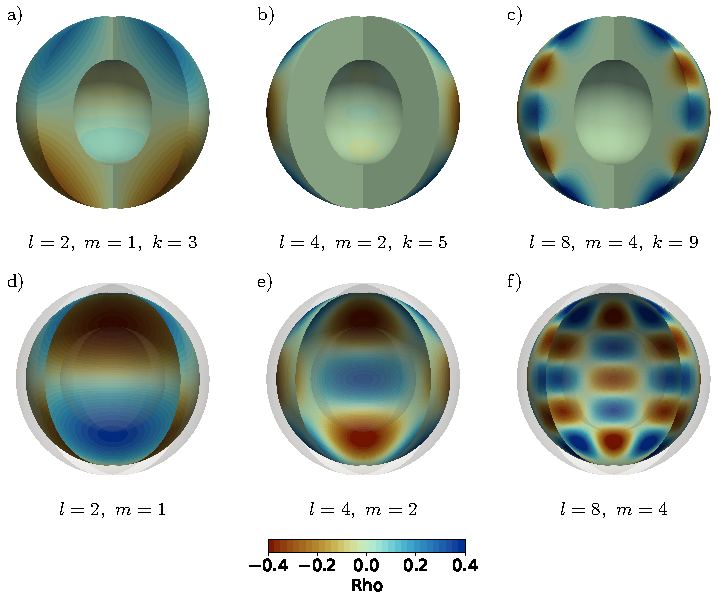
\includegraphics[width=0.98\linewidth]{figure_2_kramer_rho_ana.pdf}
    \caption{Analytical density fields. The upper row shows smooth forcing
    labelled by \((l,m,k)\). The lower row shows delta-function forcing on
    \(R_{\mathrm{int}}=2.0\), labelled only by \((l,m)\) because the delta
    forcing does not depend on the smooth radial exponent \(k\).}
    \label{fig:kramer_density_fields}
\end{figure}

\section{Numerical Setup}

The benchmark is implemented in \citetalias{Moresi2025}, a finite-element
geodynamics framework built on PETSc \citep{osti_2337606} with symbolic problem
specification in Python. The spherical-shell meshes are generated through the
Gmsh meshing backend \citep{Geuzaine2009}. The calculations use quadratic
velocity and continuous linear pressure finite elements on tetrahedral meshes,
i.e. a \(P_2\times P_1\) Taylor--Hood pair. For sufficiently smooth Stokes
solutions, this mixed pair is expected to give third-order velocity
convergence and second-order pressure convergence in volume \(L_2\) norms
\citep{girault1986,boffi2013}.

Mesh resolution is reported using the characteristic cell size
\[
  h=1/8,\;1/16,\;1/32,\;1/64 .
\]
Free-slip boundary conditions are imposed weakly, while zero-slip cases use
essential velocity constraints. Solver tolerances are chosen so that the
reported errors are dominated by discretisation rather than by linear-solver
residuals. The pressure is determined only up to an additive constant, so the
numerical and analytical pressure fields are compared after applying the same
mean-pressure gauge.

\section{Error Metrics}

Volume errors are measured with relative \(L_2\) norms. For a numerical scalar
or vector quantity \(q_h\), with analytical reference \(q^*\), the error is
\begin{equation}
  E_{L_2}^{\mathrm{rel}}(q)
  =
  \left(
  \frac{\int_\Omega |q_h-q^*|^2\,\mathrm{d}\Omega}
       {\int_\Omega |q^*|^2\,\mathrm{d}\Omega}
  \right)^{1/2}.
\end{equation}
Boundary diagnostics use the same relative norm on the inner or outer spherical
surface. We write these surfaces as \(\Gamma_{\mathrm{inner}}\) and
\(\Gamma_{\mathrm{outer}}\), so the table and figure labels use
\(E_{L_2,\Gamma_{\mathrm{inner}}}^{\mathrm{rel}}(\cdot)\) and
\(E_{L_2,\Gamma_{\mathrm{outer}}}^{\mathrm{rel}}(\cdot)\):
\begin{equation}
  E_{L_2,\Gamma}^{\mathrm{rel}}(q)
  =
  \left(
  \frac{\int_\Gamma |q_h-q^*|^2\,\mathrm{d}\Gamma}
       {\int_\Gamma |q^*|^2\,\mathrm{d}\Gamma}
  \right)^{1/2}.
\end{equation}
Observed convergence rates are computed from successive mesh refinements as
\begin{equation}
  \alpha
  =
  \frac{\log(E_{h_1}/E_{h_2})}{\log(h_1/h_2)} ,
\end{equation}
which reduces to \(\alpha=\log_2(E_{h}/E_{h/2})\) for the refinements used
here.

\section{Results}

\subsection{Volume Velocity and Pressure Errors}

For smooth Stokes solutions, a \(P_2\times P_1\) Taylor--Hood method with
accurately represented curved geometry is expected to approach third-order
velocity convergence and second-order pressure convergence in the \(L_2\) norm
\citep{girault1986,boffi2013}. The \citetalias{Moresi2025} smooth spherical
cases reproduce the second-order pressure trend but do not reach the ideal
third-order velocity rate over the tested resolutions. Case 2, with smooth
forcing and free-slip boundaries, gives velocity rates mostly between 1.9 and
2.1. Case 4, with smooth forcing and zero-slip boundaries, is similarly close
to second order, apart from higher coarse-grid pre-asymptotic rates for some
higher spherical harmonics.

The delta-function cases reproduce the reduced regularity trend reported by
\citetalias{kramer2021}. In Cases 1 and 3, the finest-grid velocity rates are
close to \(O(h^{1.5})\), while pressure rates are close to \(O(h^{0.5})\).
This behaviour is expected because the interface-localised forcing limits the
regularity of both velocity gradients and pressure. It is therefore a
benchmark feature rather than a solver failure.

\begin{figure}[H]
    \centering
    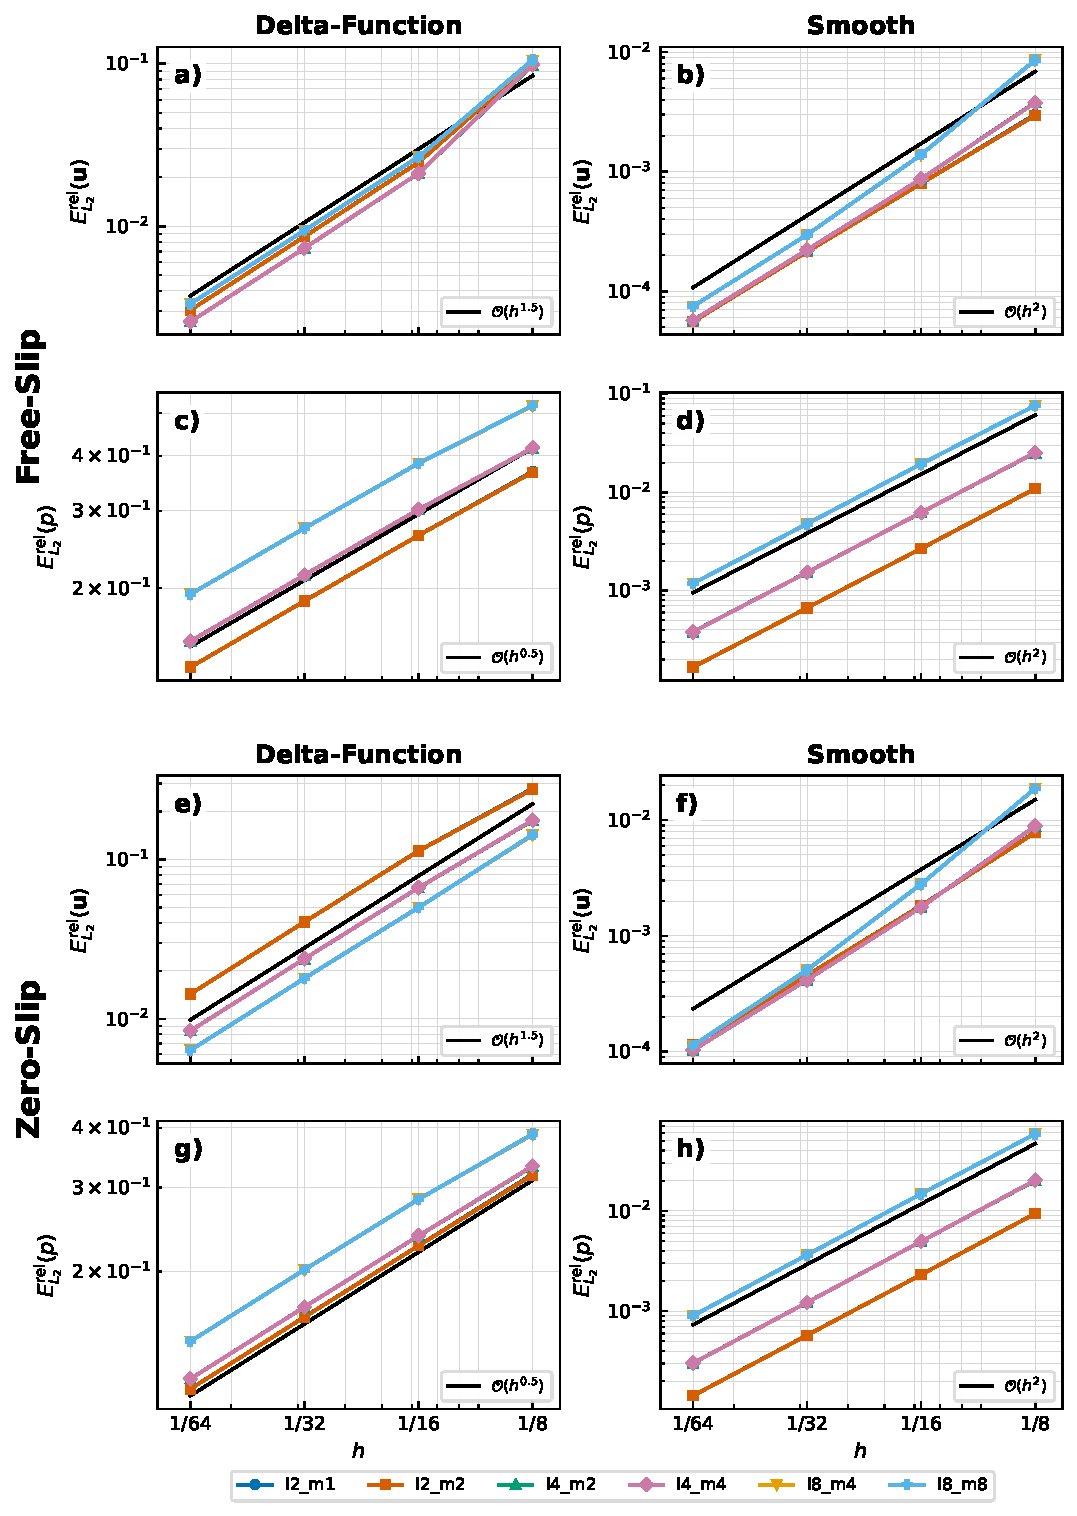
\includegraphics[height=0.72\textheight,keepaspectratio]{figure_4_kramer_spherical_convergence.pdf}
    \caption{Velocity and pressure convergence. Reference slopes distinguish smooth-solution expectations from the
    reduced rates associated with delta-function forcing. Note that all cases
    with smooth forcing are run at \(k=l+1\).}
    \label{fig:kramer_velocity_pressure_convergence}
\end{figure}

The numerical values and pairwise rates for
Fig.~\ref{fig:kramer_velocity_pressure_convergence} are listed in
Tables~\ref{tab:kramer_spherical_volume_convergence_start}--\ref{tab:kramer_spherical_volume_convergence_end}.

\begin{benchmarklandscape}
\begin{table}[p]
\centering
\caption{Case 1: free-slip, delta-function forcing (1 of 2).}
\label{tab:kramer_spherical_volume_convergence_start}
\benchmarktablefont
\setlength{\tabcolsep}{3.2pt}
\fitwidth{%
\begin{tabular}{ccccccccccccc}
\toprule
\multirow{2}{*}{$h$} & \multicolumn{4}{c}{$l=2,\,m=1$} & \multicolumn{4}{c}{$l=2,\,m=2$} & \multicolumn{4}{c}{$l=4,\,m=2$} \\
\cmidrule(lr){2-5}
\cmidrule(lr){6-9}
\cmidrule(lr){10-13}
 & $E_{L_2}^{\mathrm{rel}}(\mathbf{u})$ & rate & $E_{L_2}^{\mathrm{rel}}(p)$ & rate & $E_{L_2}^{\mathrm{rel}}(\mathbf{u})$ & rate & $E_{L_2}^{\mathrm{rel}}(p)$ & rate & $E_{L_2}^{\mathrm{rel}}(\mathbf{u})$ & rate & $E_{L_2}^{\mathrm{rel}}(p)$ & rate \\
\midrule
$1/8$ & \num{1.034e-01} & -- & \num{3.683e-01} & -- & \num{1.024e-01} & -- & \num{3.669e-01} & -- & \num{9.793e-02} & -- & \num{4.161e-01} & -- \\
$1/16$ & \num{2.473e-02} & 2.06 & \num{2.636e-01} & 0.48 & \num{2.470e-02} & 2.05 & \num{2.635e-01} & 0.48 & \num{2.117e-02} & 2.21 & \num{3.017e-01} & 0.46 \\
$1/32$ & \num{8.648e-03} & 1.52 & \num{1.869e-01} & 0.50 & \num{8.644e-03} & 1.51 & \num{1.869e-01} & 0.50 & \num{7.336e-03} & 1.53 & \num{2.142e-01} & 0.49 \\
$1/64$ & \num{3.053e-03} & 1.50 & \num{1.321e-01} & 0.50 & \num{3.052e-03} & 1.50 & \num{1.321e-01} & 0.50 & \num{2.591e-03} & 1.50 & \num{1.515e-01} & 0.50 \\
\bottomrule
\end{tabular}%
}
\end{table}

\begin{table}[p]
\centering
\caption{Case 1: free-slip, delta-function forcing (2 of 2).}
\benchmarktablefont
\setlength{\tabcolsep}{3.2pt}
\fitwidth{%
\begin{tabular}{ccccccccccccc}
\toprule
\multirow{2}{*}{$h$} & \multicolumn{4}{c}{$l=4,\,m=4$} & \multicolumn{4}{c}{$l=8,\,m=4$} & \multicolumn{4}{c}{$l=8,\,m=8$} \\
\cmidrule(lr){2-5}
\cmidrule(lr){6-9}
\cmidrule(lr){10-13}
 & $E_{L_2}^{\mathrm{rel}}(\mathbf{u})$ & rate & $E_{L_2}^{\mathrm{rel}}(p)$ & rate & $E_{L_2}^{\mathrm{rel}}(\mathbf{u})$ & rate & $E_{L_2}^{\mathrm{rel}}(p)$ & rate & $E_{L_2}^{\mathrm{rel}}(\mathbf{u})$ & rate & $E_{L_2}^{\mathrm{rel}}(p)$ & rate \\
\midrule
$1/8$ & \num{9.858e-02} & -- & \num{4.169e-01} & -- & \num{1.045e-01} & -- & \num{5.192e-01} & -- & \num{1.055e-01} & -- & \num{5.206e-01} & -- \\
$1/16$ & \num{2.119e-02} & 2.22 & \num{3.019e-01} & 0.47 & \num{2.674e-02} & 1.97 & \num{3.846e-01} & 0.43 & \num{2.666e-02} & 1.98 & \num{3.843e-01} & 0.44 \\
$1/32$ & \num{7.335e-03} & 1.53 & \num{2.142e-01} & 0.50 & \num{9.438e-03} & 1.50 & \num{2.738e-01} & 0.49 & \num{9.420e-03} & 1.50 & \num{2.737e-01} & 0.49 \\
$1/64$ & \num{2.589e-03} & 1.50 & \num{1.514e-01} & 0.50 & \num{3.336e-03} & 1.50 & \num{1.938e-01} & 0.50 & \num{3.333e-03} & 1.50 & \num{1.937e-01} & 0.50 \\
\bottomrule
\end{tabular}%
}
\end{table}

\begin{table}[p]
\centering
\caption{Case 2: free-slip, smooth forcing (1 of 2).}
\benchmarktablefont
\setlength{\tabcolsep}{3.2pt}
\fitwidth{%
\begin{tabular}{ccccccccccccc}
\toprule
\multirow{2}{*}{$h$} & \multicolumn{4}{c}{$l=2,\,m=1,\,k=3$} & \multicolumn{4}{c}{$l=2,\,m=2,\,k=3$} & \multicolumn{4}{c}{$l=4,\,m=2,\,k=5$} \\
\cmidrule(lr){2-5}
\cmidrule(lr){6-9}
\cmidrule(lr){10-13}
 & $E_{L_2}^{\mathrm{rel}}(\mathbf{u})$ & rate & $E_{L_2}^{\mathrm{rel}}(p)$ & rate & $E_{L_2}^{\mathrm{rel}}(\mathbf{u})$ & rate & $E_{L_2}^{\mathrm{rel}}(p)$ & rate & $E_{L_2}^{\mathrm{rel}}(\mathbf{u})$ & rate & $E_{L_2}^{\mathrm{rel}}(p)$ & rate \\
\midrule
$1/8$ & \num{3.011e-03} & -- & \num{1.090e-02} & -- & \num{2.964e-03} & -- & \num{1.088e-02} & -- & \num{3.803e-03} & -- & \num{2.519e-02} & -- \\
$1/16$ & \num{7.961e-04} & 1.92 & \num{2.681e-03} & 2.02 & \num{7.957e-04} & 1.90 & \num{2.680e-03} & 2.02 & \num{8.684e-04} & 2.13 & \num{6.219e-03} & 2.02 \\
$1/32$ & \num{2.145e-04} & 1.89 & \num{6.681e-04} & 2.00 & \num{2.145e-04} & 1.89 & \num{6.678e-04} & 2.00 & \num{2.221e-04} & 1.97 & \num{1.536e-03} & 2.02 \\
$1/64$ & \num{5.570e-05} & 1.95 & \num{1.669e-04} & 2.00 & \num{5.568e-05} & 1.95 & \num{1.667e-04} & 2.00 & \num{5.706e-05} & 1.96 & \num{3.813e-04} & 2.01 \\
\bottomrule
\end{tabular}%
}
\end{table}

\begin{table}[p]
\centering
\caption{Case 2: free-slip, smooth forcing (2 of 2).}
\benchmarktablefont
\setlength{\tabcolsep}{3.2pt}
\fitwidth{%
\begin{tabular}{ccccccccccccc}
\toprule
\multirow{2}{*}{$h$} & \multicolumn{4}{c}{$l=4,\,m=4,\,k=5$} & \multicolumn{4}{c}{$l=8,\,m=4,\,k=9$} & \multicolumn{4}{c}{$l=8,\,m=8,\,k=9$} \\
\cmidrule(lr){2-5}
\cmidrule(lr){6-9}
\cmidrule(lr){10-13}
 & $E_{L_2}^{\mathrm{rel}}(\mathbf{u})$ & rate & $E_{L_2}^{\mathrm{rel}}(p)$ & rate & $E_{L_2}^{\mathrm{rel}}(\mathbf{u})$ & rate & $E_{L_2}^{\mathrm{rel}}(p)$ & rate & $E_{L_2}^{\mathrm{rel}}(\mathbf{u})$ & rate & $E_{L_2}^{\mathrm{rel}}(p)$ & rate \\
\midrule
$1/8$ & \num{3.778e-03} & -- & \num{2.534e-02} & -- & \num{8.580e-03} & -- & \num{7.633e-02} & -- & \num{8.597e-03} & -- & \num{7.634e-02} & -- \\
$1/16$ & \num{8.697e-04} & 2.12 & \num{6.221e-03} & 2.03 & \num{1.384e-03} & 2.63 & \num{1.937e-02} & 1.98 & \num{1.387e-03} & 2.63 & \num{1.940e-02} & 1.98 \\
$1/32$ & \num{2.221e-04} & 1.97 & \num{1.534e-03} & 2.02 & \num{2.969e-04} & 2.22 & \num{4.787e-03} & 2.02 & \num{2.968e-04} & 2.22 & \num{4.776e-03} & 2.02 \\
$1/64$ & \num{5.702e-05} & 1.96 & \num{3.803e-04} & 2.01 & \num{7.478e-05} & 1.99 & \num{1.184e-03} & 2.02 & \num{7.484e-05} & 1.99 & \num{1.183e-03} & 2.01 \\
\bottomrule
\end{tabular}%
}
\end{table}

\begin{table}[p]
\centering
\caption{Case 3: zero-slip, delta-function forcing (1 of 2).}
\benchmarktablefont
\setlength{\tabcolsep}{3.2pt}
\fitwidth{%
\begin{tabular}{ccccccccccccc}
\toprule
\multirow{2}{*}{$h$} & \multicolumn{4}{c}{$l=2,\,m=1$} & \multicolumn{4}{c}{$l=2,\,m=2$} & \multicolumn{4}{c}{$l=4,\,m=2$} \\
\cmidrule(lr){2-5}
\cmidrule(lr){6-9}
\cmidrule(lr){10-13}
 & $E_{L_2}^{\mathrm{rel}}(\mathbf{u})$ & rate & $E_{L_2}^{\mathrm{rel}}(p)$ & rate & $E_{L_2}^{\mathrm{rel}}(\mathbf{u})$ & rate & $E_{L_2}^{\mathrm{rel}}(p)$ & rate & $E_{L_2}^{\mathrm{rel}}(\mathbf{u})$ & rate & $E_{L_2}^{\mathrm{rel}}(p)$ & rate \\
\midrule
$1/8$ & \num{2.791e-01} & -- & \num{3.198e-01} & -- & \num{2.762e-01} & -- & \num{3.185e-01} & -- & \num{1.757e-01} & -- & \num{3.320e-01} & -- \\
$1/16$ & \num{1.133e-01} & 1.30 & \num{2.265e-01} & 0.50 & \num{1.131e-01} & 1.29 & \num{2.264e-01} & 0.49 & \num{6.647e-02} & 1.40 & \num{2.375e-01} & 0.48 \\
$1/32$ & \num{4.060e-02} & 1.48 & \num{1.606e-01} & 0.50 & \num{4.058e-02} & 1.48 & \num{1.605e-01} & 0.50 & \num{2.382e-02} & 1.48 & \num{1.685e-01} & 0.49 \\
$1/64$ & \num{1.434e-02} & 1.50 & \num{1.135e-01} & 0.50 & \num{1.434e-02} & 1.50 & \num{1.135e-01} & 0.50 & \num{8.421e-03} & 1.50 & \num{1.192e-01} & 0.50 \\
\bottomrule
\end{tabular}%
}
\end{table}

\begin{table}[p]
\centering
\caption{Case 3: zero-slip, delta-function forcing (2 of 2).}
\benchmarktablefont
\setlength{\tabcolsep}{3.2pt}
\fitwidth{%
\begin{tabular}{ccccccccccccc}
\toprule
\multirow{2}{*}{$h$} & \multicolumn{4}{c}{$l=4,\,m=4$} & \multicolumn{4}{c}{$l=8,\,m=4$} & \multicolumn{4}{c}{$l=8,\,m=8$} \\
\cmidrule(lr){2-5}
\cmidrule(lr){6-9}
\cmidrule(lr){10-13}
 & $E_{L_2}^{\mathrm{rel}}(\mathbf{u})$ & rate & $E_{L_2}^{\mathrm{rel}}(p)$ & rate & $E_{L_2}^{\mathrm{rel}}(\mathbf{u})$ & rate & $E_{L_2}^{\mathrm{rel}}(p)$ & rate & $E_{L_2}^{\mathrm{rel}}(\mathbf{u})$ & rate & $E_{L_2}^{\mathrm{rel}}(p)$ & rate \\
\midrule
$1/8$ & \num{1.765e-01} & -- & \num{3.326e-01} & -- & \num{1.422e-01} & -- & \num{3.871e-01} & -- & \num{1.432e-01} & -- & \num{3.882e-01} & -- \\
$1/16$ & \num{6.656e-02} & 1.41 & \num{2.375e-01} & 0.49 & \num{5.011e-02} & 1.51 & \num{2.834e-01} & 0.45 & \num{4.997e-02} & 1.52 & \num{2.832e-01} & 0.46 \\
$1/32$ & \num{2.382e-02} & 1.48 & \num{1.685e-01} & 0.50 & \num{1.800e-02} & 1.48 & \num{2.018e-01} & 0.49 & \num{1.796e-02} & 1.48 & \num{2.017e-01} & 0.49 \\
$1/64$ & \num{8.415e-03} & 1.50 & \num{1.192e-01} & 0.50 & \num{6.366e-03} & 1.50 & \num{1.428e-01} & 0.50 & \num{6.359e-03} & 1.50 & \num{1.427e-01} & 0.50 \\
\bottomrule
\end{tabular}%
}
\end{table}

\begin{table}[p]
\centering
\caption{Case 4: zero-slip, smooth forcing (1 of 2).}
\benchmarktablefont
\setlength{\tabcolsep}{3.2pt}
\fitwidth{%
\begin{tabular}{ccccccccccccc}
\toprule
\multirow{2}{*}{$h$} & \multicolumn{4}{c}{$l=2,\,m=1,\,k=3$} & \multicolumn{4}{c}{$l=2,\,m=2,\,k=3$} & \multicolumn{4}{c}{$l=4,\,m=2,\,k=5$} \\
\cmidrule(lr){2-5}
\cmidrule(lr){6-9}
\cmidrule(lr){10-13}
 & $E_{L_2}^{\mathrm{rel}}(\mathbf{u})$ & rate & $E_{L_2}^{\mathrm{rel}}(p)$ & rate & $E_{L_2}^{\mathrm{rel}}(\mathbf{u})$ & rate & $E_{L_2}^{\mathrm{rel}}(p)$ & rate & $E_{L_2}^{\mathrm{rel}}(\mathbf{u})$ & rate & $E_{L_2}^{\mathrm{rel}}(p)$ & rate \\
\midrule
$1/8$ & \num{7.826e-03} & -- & \num{9.412e-03} & -- & \num{7.788e-03} & -- & \num{9.399e-03} & -- & \num{8.891e-03} & -- & \num{2.009e-02} & -- \\
$1/16$ & \num{1.826e-03} & 2.10 & \num{2.313e-03} & 2.02 & \num{1.820e-03} & 2.10 & \num{2.311e-03} & 2.02 & \num{1.764e-03} & 2.33 & \num{4.960e-03} & 2.02 \\
$1/32$ & \num{4.559e-04} & 2.00 & \num{5.754e-04} & 2.01 & \num{4.553e-04} & 2.00 & \num{5.744e-04} & 2.01 & \num{4.164e-04} & 2.08 & \num{1.223e-03} & 2.02 \\
$1/64$ & \num{1.141e-04} & 2.00 & \num{1.435e-04} & 2.00 & \num{1.140e-04} & 2.00 & \num{1.432e-04} & 2.00 & \num{1.029e-04} & 2.02 & \num{3.032e-04} & 2.01 \\
\bottomrule
\end{tabular}%
}
\end{table}

\begin{table}[p]
\centering
\caption{Case 4: zero-slip, smooth forcing (2 of 2).}
\label{tab:kramer_spherical_volume_convergence_end}
\benchmarktablefont
\setlength{\tabcolsep}{3.2pt}
\fitwidth{%
\begin{tabular}{ccccccccccccc}
\toprule
\multirow{2}{*}{$h$} & \multicolumn{4}{c}{$l=4,\,m=4,\,k=5$} & \multicolumn{4}{c}{$l=8,\,m=4,\,k=9$} & \multicolumn{4}{c}{$l=8,\,m=8,\,k=9$} \\
\cmidrule(lr){2-5}
\cmidrule(lr){6-9}
\cmidrule(lr){10-13}
 & $E_{L_2}^{\mathrm{rel}}(\mathbf{u})$ & rate & $E_{L_2}^{\mathrm{rel}}(p)$ & rate & $E_{L_2}^{\mathrm{rel}}(\mathbf{u})$ & rate & $E_{L_2}^{\mathrm{rel}}(p)$ & rate & $E_{L_2}^{\mathrm{rel}}(\mathbf{u})$ & rate & $E_{L_2}^{\mathrm{rel}}(p)$ & rate \\
\midrule
$1/8$ & \num{8.873e-03} & -- & \num{2.021e-02} & -- & \num{1.873e-02} & -- & \num{5.851e-02} & -- & \num{1.875e-02} & -- & \num{5.853e-02} & -- \\
$1/16$ & \num{1.763e-03} & 2.33 & \num{4.960e-03} & 2.03 & \num{2.801e-03} & 2.74 & \num{1.477e-02} & 1.99 & \num{2.798e-03} & 2.74 & \num{1.480e-02} & 1.98 \\
$1/32$ & \num{4.164e-04} & 2.08 & \num{1.222e-03} & 2.02 & \num{5.075e-04} & 2.46 & \num{3.645e-03} & 2.02 & \num{5.073e-04} & 2.46 & \num{3.635e-03} & 2.03 \\
$1/64$ & \num{1.028e-04} & 2.02 & \num{3.026e-04} & 2.01 & \num{1.130e-04} & 2.17 & \num{9.003e-04} & 2.02 & \num{1.129e-04} & 2.17 & \num{8.992e-04} & 2.02 \\
\bottomrule
\end{tabular}%
}
\end{table}
\end{benchmarklandscape}

\subsection{Boundary Velocity and Radial Normal Stress}

Boundary metrics are evaluated on the inner and outer spherical surfaces for
Case 1, the free-slip delta-function benchmark. This is the most demanding of
the tested boundary diagnostics because the forcing is singular and the
free-slip condition is imposed on curved boundaries. Boundary velocity errors
fall rapidly on the coarse refinements, with outer-boundary rates near third to
fourth order. On the finest refinement the inner-boundary velocity rates reduce
to approximately 2.3--2.6, while the outer boundary remains higher for the
lower spherical harmonics.

The radial normal stress \(\sigma_{rr}\) is more sensitive than velocity because
it combines pressure and velocity-gradient errors and is then evaluated on a
curved boundary. The stress errors decrease systematically but show more
variable rates than the volume norms. Coarse-grid rates are partly
pre-asymptotic, whereas finest-grid rates are closer to first-to-second order.
This is consistent with the singular forcing, continuous pressure
approximation, derivative recovery, boundary quadrature, and weak free-slip
enforcement all contributing to the boundary stress error.

\begin{figure}[H]
    \centering
    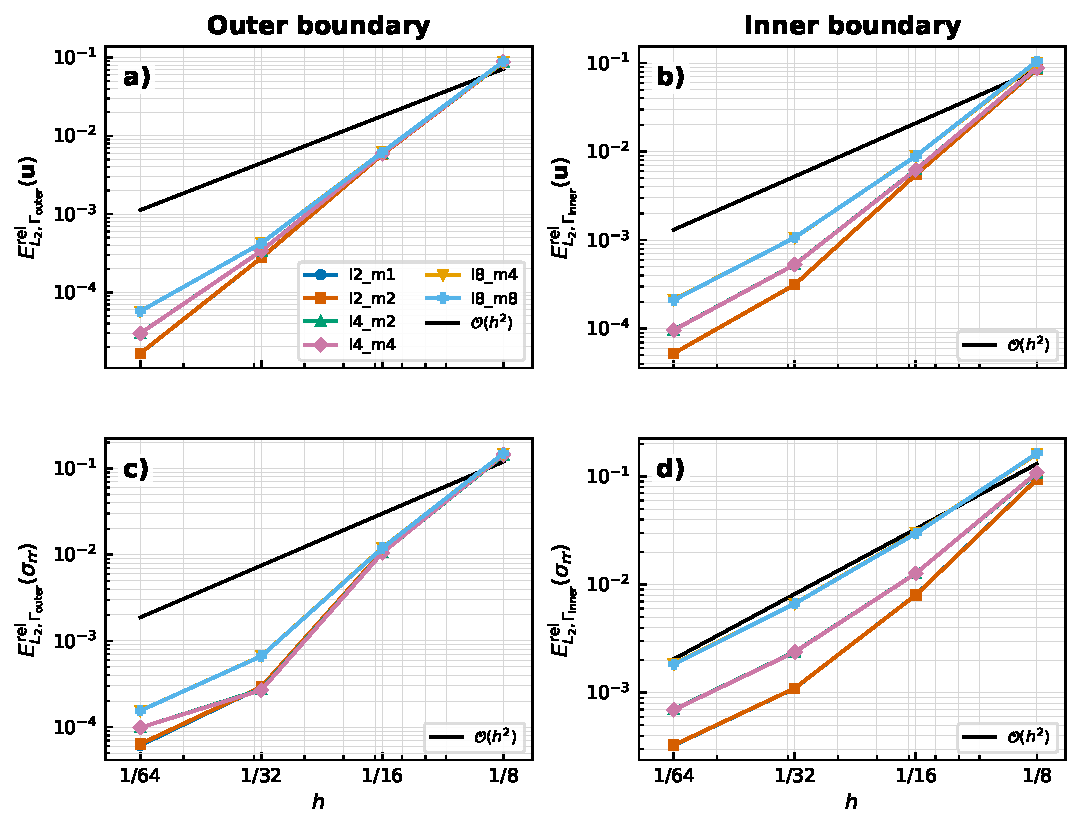
\includegraphics[width=0.98\linewidth]{figure_7_kramer_boundary_convergence.pdf}
    \caption{Boundary velocity and radial normal-stress convergence on the
    inner and outer spherical boundaries for Case 1.}
    \label{fig:kramer_boundary_convergence}
\end{figure}

The corresponding boundary velocity and radial normal-stress values are listed
in Tables~\ref{tab:kramer_spherical_boundary_convergence_start}--\ref{tab:kramer_spherical_boundary_convergence_end}.

\begin{benchmarklandscape}

\begin{table}[p]
\centering
\caption{Case 1 boundary velocity convergence (1 of 2).}
\label{tab:kramer_spherical_boundary_convergence_start}
\benchmarktablefont
\setlength{\tabcolsep}{3.2pt}
\fitwidth{%
\begin{tabular}{ccccccccccccc}
\toprule
\multirow{2}{*}{$h$} & \multicolumn{4}{c}{$l=2,\,m=1$} & \multicolumn{4}{c}{$l=2,\,m=2$} & \multicolumn{4}{c}{$l=4,\,m=2$} \\
\cmidrule(lr){2-5}
\cmidrule(lr){6-9}
\cmidrule(lr){10-13}
 & $E_{L_2,\Gamma_{\mathrm{outer}}}^{\mathrm{rel}}(\mathbf{u})$ & rate & $E_{L_2,\Gamma_{\mathrm{inner}}}^{\mathrm{rel}}(\mathbf{u})$ & rate & $E_{L_2,\Gamma_{\mathrm{outer}}}^{\mathrm{rel}}(\mathbf{u})$ & rate & $E_{L_2,\Gamma_{\mathrm{inner}}}^{\mathrm{rel}}(\mathbf{u})$ & rate & $E_{L_2,\Gamma_{\mathrm{outer}}}^{\mathrm{rel}}(\mathbf{u})$ & rate & $E_{L_2,\Gamma_{\mathrm{inner}}}^{\mathrm{rel}}(\mathbf{u})$ & rate \\
\midrule
$1/8$ & \num{8.877e-02} & -- & \num{8.511e-02} & -- & \num{8.782e-02} & -- & \num{8.478e-02} & -- & \num{8.760e-02} & -- & \num{8.756e-02} & -- \\
$1/16$ & \num{5.788e-03} & 3.94 & \num{5.496e-03} & 3.95 & \num{5.786e-03} & 3.92 & \num{5.487e-03} & 3.95 & \num{5.942e-03} & 3.88 & \num{6.265e-03} & 3.80 \\
$1/32$ & \num{2.762e-04} & 4.39 & \num{3.142e-04} & 4.13 & \num{2.764e-04} & 4.39 & \num{3.145e-04} & 4.12 & \num{3.383e-04} & 4.13 & \num{5.312e-04} & 3.56 \\
$1/64$ & \num{1.653e-05} & 4.06 & \num{5.257e-05} & 2.58 & \num{1.654e-05} & 4.06 & \num{5.257e-05} & 2.58 & \num{2.984e-05} & 3.50 & \num{9.674e-05} & 2.46 \\
\bottomrule
\end{tabular}%
}
\end{table}

\begin{table}[p]
\centering
\caption{Case 1 boundary velocity convergence (2 of 2).}
\benchmarktablefont
\setlength{\tabcolsep}{3.2pt}
\fitwidth{%
\begin{tabular}{ccccccccccccc}
\toprule
\multirow{2}{*}{$h$} & \multicolumn{4}{c}{$l=4,\,m=4$} & \multicolumn{4}{c}{$l=8,\,m=4$} & \multicolumn{4}{c}{$l=8,\,m=8$} \\
\cmidrule(lr){2-5}
\cmidrule(lr){6-9}
\cmidrule(lr){10-13}
 & $E_{L_2,\Gamma_{\mathrm{outer}}}^{\mathrm{rel}}(\mathbf{u})$ & rate & $E_{L_2,\Gamma_{\mathrm{inner}}}^{\mathrm{rel}}(\mathbf{u})$ & rate & $E_{L_2,\Gamma_{\mathrm{outer}}}^{\mathrm{rel}}(\mathbf{u})$ & rate & $E_{L_2,\Gamma_{\mathrm{inner}}}^{\mathrm{rel}}(\mathbf{u})$ & rate & $E_{L_2,\Gamma_{\mathrm{outer}}}^{\mathrm{rel}}(\mathbf{u})$ & rate & $E_{L_2,\Gamma_{\mathrm{inner}}}^{\mathrm{rel}}(\mathbf{u})$ & rate \\
\midrule
$1/8$ & \num{8.839e-02} & -- & \num{8.836e-02} & -- & \num{8.885e-02} & -- & \num{1.018e-01} & -- & \num{8.986e-02} & -- & \num{1.049e-01} & -- \\
$1/16$ & \num{5.913e-03} & 3.90 & \num{6.234e-03} & 3.83 & \num{6.205e-03} & 3.84 & \num{8.936e-03} & 3.51 & \num{6.170e-03} & 3.86 & \num{8.911e-03} & 3.56 \\
$1/32$ & \num{3.382e-04} & 4.13 & \num{5.296e-04} & 3.56 & \num{4.244e-04} & 3.87 & \num{1.069e-03} & 3.06 & \num{4.239e-04} & 3.86 & \num{1.072e-03} & 3.05 \\
$1/64$ & \num{2.976e-05} & 3.51 & \num{9.631e-05} & 2.46 & \num{5.715e-05} & 2.89 & \num{2.117e-04} & 2.34 & \num{5.713e-05} & 2.89 & \num{2.100e-04} & 2.35 \\
\bottomrule
\end{tabular}%
}
\end{table}

\begin{table}[p]
\centering
\caption{Case 1 boundary radial-stress convergence (1 of 2).}
\benchmarktablefont
\setlength{\tabcolsep}{3.2pt}
\fitwidth{%
\begin{tabular}{ccccccccccccc}
\toprule
\multirow{2}{*}{$h$} & \multicolumn{4}{c}{$l=2,\,m=1$} & \multicolumn{4}{c}{$l=2,\,m=2$} & \multicolumn{4}{c}{$l=4,\,m=2$} \\
\cmidrule(lr){2-5}
\cmidrule(lr){6-9}
\cmidrule(lr){10-13}
 & $E_{L_2,\Gamma_{\mathrm{outer}}}^{\mathrm{rel}}(\sigma_{rr})$ & rate & $E_{L_2,\Gamma_{\mathrm{inner}}}^{\mathrm{rel}}(\sigma_{rr})$ & rate & $E_{L_2,\Gamma_{\mathrm{outer}}}^{\mathrm{rel}}(\sigma_{rr})$ & rate & $E_{L_2,\Gamma_{\mathrm{inner}}}^{\mathrm{rel}}(\sigma_{rr})$ & rate & $E_{L_2,\Gamma_{\mathrm{outer}}}^{\mathrm{rel}}(\sigma_{rr})$ & rate & $E_{L_2,\Gamma_{\mathrm{inner}}}^{\mathrm{rel}}(\sigma_{rr})$ & rate \\
\midrule
$1/8$ & \num{1.500e-01} & -- & \num{9.413e-02} & -- & \num{1.458e-01} & -- & \num{9.370e-02} & -- & \num{1.424e-01} & -- & \num{1.073e-01} & -- \\
$1/16$ & \num{1.096e-02} & 3.77 & \num{8.041e-03} & 3.55 & \num{1.095e-02} & 3.74 & \num{8.024e-03} & 3.55 & \num{1.054e-02} & 3.76 & \num{1.272e-02} & 3.08 \\
$1/32$ & \num{2.905e-04} & 5.24 & \num{1.100e-03} & 2.87 & \num{2.920e-04} & 5.23 & \num{1.102e-03} & 2.86 & \num{2.737e-04} & 5.27 & \num{2.392e-03} & 2.41 \\
$1/64$ & \num{6.125e-05} & 2.25 & \num{3.258e-04} & 1.76 & \num{6.364e-05} & 2.20 & \num{3.276e-04} & 1.75 & \num{9.848e-05} & 1.47 & \num{6.990e-04} & 1.77 \\
\bottomrule
\end{tabular}%
}
\end{table}

\begin{table}[p]
\centering
\caption{Case 1 boundary radial-stress convergence (2 of 2).}
\label{tab:kramer_spherical_boundary_convergence_end}
\benchmarktablefont
\setlength{\tabcolsep}{3.2pt}
\fitwidth{%
\begin{tabular}{ccccccccccccc}
\toprule
\multirow{2}{*}{$h$} & \multicolumn{4}{c}{$l=4,\,m=4$} & \multicolumn{4}{c}{$l=8,\,m=4$} & \multicolumn{4}{c}{$l=8,\,m=8$} \\
\cmidrule(lr){2-5}
\cmidrule(lr){6-9}
\cmidrule(lr){10-13}
 & $E_{L_2,\Gamma_{\mathrm{outer}}}^{\mathrm{rel}}(\sigma_{rr})$ & rate & $E_{L_2,\Gamma_{\mathrm{inner}}}^{\mathrm{rel}}(\sigma_{rr})$ & rate & $E_{L_2,\Gamma_{\mathrm{outer}}}^{\mathrm{rel}}(\sigma_{rr})$ & rate & $E_{L_2,\Gamma_{\mathrm{inner}}}^{\mathrm{rel}}(\sigma_{rr})$ & rate & $E_{L_2,\Gamma_{\mathrm{outer}}}^{\mathrm{rel}}(\sigma_{rr})$ & rate & $E_{L_2,\Gamma_{\mathrm{inner}}}^{\mathrm{rel}}(\sigma_{rr})$ & rate \\
\midrule
$1/8$ & \num{1.447e-01} & -- & \num{1.083e-01} & -- & \num{1.489e-01} & -- & \num{1.618e-01} & -- & \num{1.499e-01} & -- & \num{1.637e-01} & -- \\
$1/16$ & \num{1.052e-02} & 3.78 & \num{1.270e-02} & 3.09 & \num{1.203e-02} & 3.63 & \num{3.009e-02} & 2.43 & \num{1.192e-02} & 3.65 & \num{2.971e-02} & 2.46 \\
$1/32$ & \num{2.683e-04} & 5.29 & \num{2.379e-03} & 2.42 & \num{6.680e-04} & 4.17 & \num{6.678e-03} & 2.17 & \num{6.658e-04} & 4.16 & \num{6.670e-03} & 2.16 \\
$1/64$ & \num{9.866e-05} & 1.44 & \num{6.942e-04} & 1.78 & \num{1.547e-04} & 2.11 & \num{1.841e-03} & 1.86 & \num{1.547e-04} & 2.11 & \num{1.831e-03} & 1.87 \\
\bottomrule
\end{tabular}%
}
\end{table}
\end{benchmarklandscape}

\section{Discussion}

The \citetalias{Moresi2025} calculations reproduce the primary
\citetalias{kramer2021} spherical-shell benchmark distinction between smooth
and delta-function forcing. Smooth pressure converges close to the expected
\(O(h^2)\) rate, and delta-function forcing reduces velocity and pressure
convergence to the expected approximate \(O(h^{1.5})\) and \(O(h^{0.5})\)
trends. These results indicate that the analytical forcing, pressure
normalisation, and mixed Stokes solve are implemented consistently.

The main discrepancy from the ideal smooth-solution expectation is velocity:
the smooth cases converge closer to second order than to the third-order
\(P_2\) \(L_2\) rate obtained by \citetalias{kramer2021} with curved/isoparametric
Fluidity calculations. The pressure result narrows the likely explanation. The
Stokes solve and smooth forcing are behaving consistently, but geometry
representation, boundary-condition enforcement, quadrature, mesh quality, or
the interaction among these terms appears to limit the velocity error before
the polynomial interpolation rate is reached.

The boundary results are intentionally more demanding than volume norms.
Radial normal stress contains pressure directly and velocity derivatives
through \(2\eta\boldsymbol{\varepsilon}(\mathbf{u})\), so it inherits pressure
regularity limits and derivative-recovery errors. Differences between inner and
outer boundary errors are therefore expected because the surfaces have
different radii, analytical amplitudes, quadrature weights, and sensitivity to
mesh geometry. Higher \((l,m)\) values further increase angular gradients and
delay asymptotic behaviour.

\conclusions

We have presented a verification study of the \citetalias{kramer2021}
spherical-shell Stokes benchmark using \citetalias{Moresi2025}. The benchmark
tests smooth and delta-function forcing, free-slip and zero-slip boundary
conditions, volume velocity and pressure errors, and boundary velocity and
radial normal-stress diagnostics. The principal conclusions are:
\begin{enumerate}
  \item \citetalias{Moresi2025} reproduces the expected contrast between
  smooth volumetric forcing and delta-function interface forcing in a
  spherical shell.
  \item Smooth pressure errors converge at approximately second order for the
  \(P_2\times P_1\) Taylor--Hood discretisation.
  \item Smooth velocity errors converge robustly but remain closer to second
  order than to the ideal third-order \(P_2\) \(L_2\) rate over the tested
  resolutions.
  \item Delta-function cases show the expected reduced convergence rates,
  approximately \(O(h^{1.5})\) for velocity and \(O(h^{0.5})\) for pressure.
  \item Boundary velocity and radial normal-stress errors decrease
  systematically, with stress recovery showing the strongest sensitivity to
  singular forcing and curved-boundary post-processing.
\end{enumerate}
Overall, the benchmark supports \citetalias{Moresi2025} spherical-shell Stokes
verification while identifying smooth-case velocity convergence and boundary
stress recovery as the most useful next diagnostics for curved geometry and
boundary-condition development.

\bibliographystyle{copernicus}
\bibliography{kramer_spherical_benchmark_article_refs}

\end{document}
